\documentclass[class=article, crop=false]{standalone}
\usepackage{tikz}
\usepackage{subcaption}
\usetikzlibrary{calc}
\usetikzlibrary {shapes.geometric}

\begin{document}
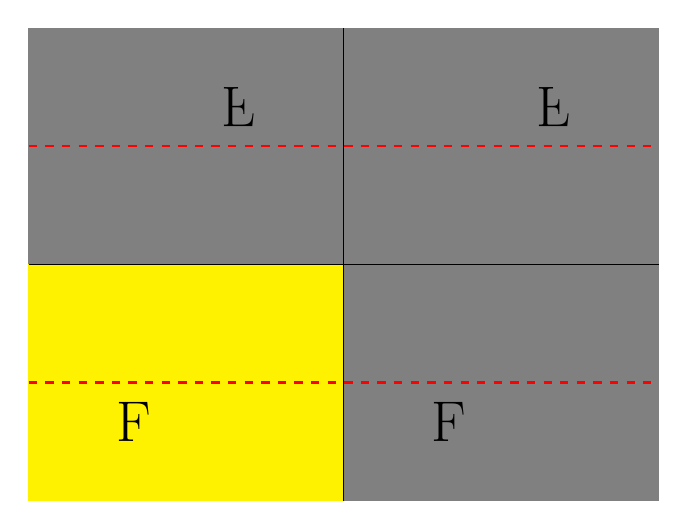
\begin{tikzpicture}
            % Define the lengths of the sides and the angle
            \def\a{4}  % length of side a
            \def\b{3}  % length of side b
            \def\angle{90}  % angle between sides a and b
            \def\s{F} % Label in center of cells


        
            % Calculate the coordinates of the points
            \coordinate (C00) at (0, 0);
            \coordinate (C10) at (\a, 0);
            \coordinate (C11) at ({\a + \b*cos(\angle)}, {\b * sin(\angle)});
            \coordinate (C01) at ({\b * cos(\angle)}, {\b * sin(\angle)});
            \coordinate (C02) at ({2*\b*cos(\angle)}, {2*\b * sin(\angle)});
            \coordinate (C12) at ({\a +2*\b * cos(\angle)}, {2*\b * sin(\angle)});
            \coordinate (C22) at ({2*\a + 2*\b * cos(\angle)}, {2*\b * sin(\angle)});
            \coordinate (C21) at ({2*\a + \b*cos(\angle)}, {\b * sin(\angle)});
            \coordinate (C20) at ({2*\a}, 0);

            \coordinate (A1) at ($(C00)!0.6666!(C11)$);
            \coordinate (A2) at ($(C11)!0.3333!(C22)$);
        
            % Draw the oblique unit cell
            \draw[fill=gray,gray] (C00) -- (C20) -- (C22) -- (C02) -- cycle;
            \draw[fill=yellow,yellow] (C00) -- (C01) -- (C11) -- (C10) -- cycle;
            \draw[] (C01) -- (C11) -- (C12);
            \draw[] (C10) -- (C11) -- (C21);
            
            % Draw chiral center
            \node at ($(C00)!0.3333!(C11)$) {\huge \s};
            \node at ($(C10)!0.3333!(C21)$) {\huge \s};
            \node[rotate=180] at ($(C11)!0.6666!(C22)$) {\reflectbox{\huge \s}};
            \node[rotate=180] at ($(C01)!0.6666!(C12)$) {\reflectbox{\huge \s}};

            % Draw mirror lines
            \draw[thick,dashed,red] ($(C00)!0.5!(C01)$) -- ($(C20)!0.5!(C21)$);
            \draw[thick,dashed,red] ($(C01)!0.5!(C02)$) -- ($(C21)!0.5!(C22)$);

            
        \end{tikzpicture}
\end{document}